\chapter{Introduction}
%In 1983, 
Two key articles published in the 1980's defined the new phenomenon of store-operated calcium entry (SOCE): \citet{Streb:1983p278} showed that stimulation with inositol (1,4,5)-trisphosphate (IP3) triggered calcium (\Ca) release from the endoplasmic reticulum (ER) and soon after, %Later, in 1986, 
\citet{Putney:1986p283}, proposed that depletion of intracellular \Ca{} concentration (\cai) signaled the plasma membrane \Ca{} entry channels to open \citep{Taylor2006}. These and other
early studies %in macrophages and Jurkat cells 
\citep{Hoth:1992p527,Zweifach1993} formed the framework for subsequent investigations of \SOCE{} in various cell types. Initially, the more popular term used was capacitive calcium entry (CCE). Over 20 years later, other major players in this story were revealed. Stromal interaction molecule 1 (STIM1), was found to affect SOC influx in an RNA interference (\rnai) based screen and identified as the ER calcium sensor \citep{Roos2005, Liou2005, Zhang2005}. Shortly thereafter the store-operated calcium channel, Orai1, was identified \citep{Feske2006, Prakriya2006, Vig2006, Zhang2006, Smyth2010}. 

There are two mammalian homologs of Orai1 -- Orai2 and Orai3 -- whose functions are not yet fully understood \citep{Roos2005,Vig2006,Taylor2006,Smyth2010}. It is possible that Orai2 and Orai3 are expressed in a tissue-specific manner. This seems to be the case with estrogen receptor-positive (ER+) breast cancer cells, which have been shown to use Orai3 as their store-operated \Ca{} channel \citep{Motiani2010, Dellis2011}. The demonstrable involvement of Orai3 in a disease state as prevalent as breast cancer, underscores the importance of further studies of these Orai channels whose function in the body is not yet understood. The presented study sets the foundation for pharmacological characterization of the Orai3 \Ca{} channel, using \droso{} S2 cells as a heterologous expression system. This system is expected to be of more general use for physiological and pharmacological studies of all Orai channels. We begin by introducing calcium signaling through store-operated channels in non-excitable cells. 



\section{Background}


\subsection{Calcium Signaling}
%Ultimately we will be looking at the effect which 2-APB has on Orai3, using cellular \Ca{} elevations as our output.   
\Ca{} is an incredibly versatile signaling molecule, affecting all parts of the cellular signaling machinery. \Ca{} signaling is critical to such processes as exocytosis, transcription, cardiac function, mitosis and apoptosis \citep{Berridge2003,Berridge2000,Gwack2007,Smyth2010}. 
The speed of these processes range from seconds to days \citep{Berridge2003}. 

Since \Ca{} can enter the cell's cytoplasm by influx at the plasma membrane or release from internal stores, such as those within the ER \citep{Berridge2003,Berridge2000,Smyth2010}, it is necessary to maintain a balance between the two pathways. This is to prevent \Ca{} from accumulating where it should not, which would activate or deactivate cellular processes at inopportune times. 
\Ca{} concentration is regulated through activation of different  ion channels.
The most studied \Ca{} ion channels in the ER are the IP3 and ryanodine receptors  (IP3R, RYR) \citep{Berridge2000, Lewis2001, WPutney:2006p130}. These channels are activated by %additional 
second messengers. %The IP3R is activated by IP3 which opens the channel, allowing release of ER \Ca{} into the cytoplasm.

``On'' mechanisms are the means by which \Ca{} is released from internal stores into the cytoplasm. ``On'' mechanisms depend on \Ca{} channels \citep{Berridge2000} which may be voltage-operated channels (VOCs), receptor-operated channels (ROCs), and/or store-operated channels (SOCs) \citep{Berridge2000}. 


``Off'' mechanisms also exist to quickly lower \cai, and this is done through various pumps and exchangers \citep{Berridge2000}. The plasma membrane \Ca -ATPase and Na$^+$/\Ca{} exchanger (if present)  move \Ca{} out of the cell, while the sarco-endoplasmic reticulum \Ca{} ATPase (SERCA) will pump \Ca{} back into the ER, replenishing the cell's internal stores \citep{Berridge2000}.

Orai1, the recently identified Calcium-Release Activated Calcium (CRAC) channel, is a store-operated \Ca{} channel \citep{Prakriya2006, Vig2006, Feske2006, Zhang2006, Smyth2010}. 
Orai3 is closely related to Orai1 \citep{Feske2006, Taylor2006, Gwack2007}, and is thought to be involved in store-operated calcium entry (SOCE). According to the Basic Local Alignment Search Tool (BLAST), Orai3 has 58\% nucleotide sequence homology with Orai1. 
%It is necessary then to understand the role that \Ca{} plays in this process.
When SOCs open they allow \Ca{} into the cytosol. This leads to \cai{} increasing from nanomolar to micromolar levels \citep{Berridge2000}. This \Ca{} is both stimulatory and inhibitory \citep{Berridge2000} since this ion acts as a signal for such a wide array of cellular processes. Spatial regulation becomes very important in allowing for control of stimulatory and inhibitory \Ca-dependent mechanisms. \Ca-binding proteins act as buffers and allow the cell to control the local \cai. Cytosolic \Ca{} buffers such as parvalbumin, calbindin-D, and calreticulin, along with \Ca{} pumps and exchangers are important in regulation of \cai{} \citep{Berridge2000}. 
The affinity which these buffers have for \Ca{} is also important. Parvalbumin, for example, has a high affinity for \Ca{} but slower binding kinetics than calbindin-D and calreticulin \cite{Berridge2003}. The different \Ca{} binding affinities allow for buffers which can modify amplitude, recovery time and diffusional range of \Ca{} %transients 
\cite{Berridge2003}. 


In addition to their buffering capacity, cytosolic \Ca{} binding proteins can also act as  \Ca{} sensors \citep{Berridge2000}.  \Ca{} sensors, such as troponin C, calmodulin, phospholipase C 
% PLC has 4 EF-hands motifs for binding Ca2+
and recoverin respond to changes in \cai. They do so with the aid of %four
 EF hand motifs and will bind \Ca{} to undergo conformational changes, and then activate downstream processes \citep{Berridge2000}. This mechanism of detecting changes in \cai{} should be emphasized, as it will become relevant for another player in the SOCE mechanism, \stim.

\subsection{Store-Operated Calcium Entry}

SOCE is an interesting, yet simple process. Broken down to its simplest form, it is a process which signals for \Ca{} to be allowed into the cell when more is needed \citep{Putney:1986p283,Berridge2000,Lewis2001}. SOCE is triggered by the loss of \Ca{} from the cell's own internal ER \Ca{} stores. ER \Ca{} sensors detect the loss of \Ca{}, migrate close to the plasma membrane (PM), and signal PM \Ca{} channels to open. This further increases the \cai{} and allows for replenishing the stores \citep{Taylor2006}, as well as providing \Ca{} necessary for various cellular processes \citep{Berridge2003,Berridge2000,Gwack2007,Smyth2010}. % A good analogy for the process would be flushing a toilet bowl. The toilet is flushed and water, analogous to \Ca, is depleted. This results in an influx of water from an external reservoir (extracellular environment). Our water will then move along a pipe, signifying our \Ca{} channel, from our external environment, eventually refilling the toilet bowl. 

Store-operated \Ca{} channels in lymphocytes are responsible for \Ca{} entering from extracellular fluid (i.e. blood) \citep{Lewis2001,Berridge2000, Gwack2007}, and lack voltage-sensitive \Ca{} channels \citep{Lioudyno2008}. T-cell receptor engagement activates the enzyme phospholipase C gamma (PLC$_\gamma$). PLC$_\gamma$ will then  hydrolyze phosphatidylinositol 4,5-bisphosphate (PIP2) in the membrane resulting in soluble IP3, and membrane-bound diacylglycerol (DAG) \citep{Berridge2000,Lewis2001}. IP3 binds to IP3R opening it and allowing \Ca{} out of the ER down its concentration gradient \citep{Smyth2010,Taylor2006,Lewis2001}. The emptying of ER \Ca{} stores is detected by \stim{} and leads to opening of the store-operated \Ca{} channels in the PM (detailed below) allowing \Ca{} into the cytosol \citep{Smyth2010,Taylor2006}. 
This sustained \Ca{} influx is necessary for gene transcription driven by nuclear factor of activated T-cells (NF-AT)  \citep{Timmerman:1996p528,Berridge2000,Lewis2001, Gwack2007}. NF-AT, a transcription factor, is activated when an immune response is necessary, and drives transcription of the IL-2 gene \citep{Timmerman:1996p528,Lewis2001,Gwack2007}. 
The importance of \Ca{} to this process is a result of NF-AT's dependence on calcineurin for activation. 

The \Ca{} influx triggered by SOCE results in \Ca{} and calmodulin binding to the protein phosphatase calcineurin, activating it. Activated calcineurin then dephosphorylates NF-AT, allowing it to move into the nucleus \citep{Timmerman:1996p528, Baksh2000}. Once inside the nucleus, NF-AT is able to bind the promoter region of interleukin and proliferation genes enabling their transcription, in effect triggering immune response \citep{Timmerman:1996p528,Berridge2000,Gwack2007}. 
Notice that for efficient NF-AT activation, the \Ca{} elevation needs to be sustained, lasting 1-2 hours \citep{Timmerman:1996p528,Berridge2000,Lewis2001}. 

%Now that we have presented a general idea of SOCE it will hopefully be easier to understand the mechanism. 
 


\section{STIM1}
% Add to Eid, J. P., A. M. Arias, et al. (2008). "The Drosophila STIM1 orthologue, dSTIM, has roles in cell fate specification and tissue patterning." BMC Dev Biol 8: 104. 
% also check last ref in this paper for original stim1, and cite it.

Stromal interaction molecule 1 (\stim), initially discovered as a membrane protein \citep{Williams2001}, was shown to be the \Ca{} sensor 
within the ER \citep{Roos2005, Liou2005, Zhang2005,Smyth2010}. The related STIM2 and \droso{} STIM (\dstim) were also discovered later \citep{Williams2001}.
STIM1 and STIM2 are single-pass transmembrane proteins \citep{Gwack2007}. Both are ER membrane localized proteins, until emptying of the ER \Ca{} store causes translocation into, or close to, the PM \citep{Gwack2007}.
%\stim{} was later shown to act as a sensor for \Ca{} within the ER \citep{Roos2005, Liou2005, Zhang2005,Smyth2010}. 

\stim{} functions as a \Ca{} sensor by binding \Ca{} with its EF hand \citep{Williams2001, Liou2005}, a motif also present in cytosolic \Ca{} sensors (see above). Upon \Ca{} depletion, ER-localized \stim{} will migrate to sites at or near the PM and bind Orai1, activating the channel. 
Once activated, Orai channels permit the flow of \Ca{} into the cell. To date, only Orai1 has been shown to be both necessary and sufficient for \Ca{} entry \citep{Feske2006, Smyth2010}.  
STIM2, a homolog of \stim, was found by one group to be an inhibitor of STIM1-mediated SOCE \citep{Soboloff2006}. 
\dstim, the \droso{} homolog of \stim, is also an important regulator of SOCE and is involved in cell fate specification and tissue patterning \citep{Eid2008}. 
%\dstim behaves similarly, associating with \dorai{} upon store-depletion.  
%\todo{add info from Luik2008}
%\todo{[not only: some STIM is constitutively in the PM (see the original Dziadek paper. This needs to be mentioned here.]}

\section{Orai3}
        
As mentioned above, Orai3 is a homolog of Orai1, the long sought after CRAC channel \citep{Feske2006,Gwack2007}. Even now, years after its discovery, the field still has a poor understanding of Orai3's native function and this is why studying Orai3 is important.

Though Orai channels behave similarly as \Ca{} entry channels, they have a different pharmacological profile. In mammalian cells, for example, interaction with the drug 2-aminoethoxydiphenyl borate (2-APB) generates different cellular responses depending on the protein to which it binds. 
While Orai1 will see slight activation upon introduction of $<$ 10 $\mu$M 2-APB, % to its cellular milieu introduction of 
higher concentrations result in deactivation \citep{Feske2006,Goto2010,Prakriya2006,Zhang2008a}, and blockade of SOCE. In contrast, Orai3 is activated by 2-APB concentrations of and above 50 $\mu$M 2-APB \citep{Goto2010,Zhang2008a}. These contrasting responses will be exploited in this study.

The Orai family of proteins displays a wide expression profile, which includes T-cells and kidney \citep{Gwack2007}. In HEK293 cells, knock down of Orai1 using siRNA reduced SOCE \citep{Gwack2007}. Knock down of Orai2 or Orai3 did not significantly affect SOCE, however \citep{Gwack2007}. These experiments in HEK cells are suggestive of Orai1's importance in initiating SOCE. As long as Orai1 is present in the membrane, SOCE will take place normally. Overexpression experiments of Orai1 showing \Ca{} influx lasting minutes support this idea \citep{Gwack2007,Zhang2008a}. \Ca{} influx on the order of hours is necessary for gene transcription, however \citep{Baksh2000}. 

%Also suggestive of this is an experiment by \citet{Gwack2007} showing that siRNA knockdown of Orai3 in HEK cells results in a 3 fold increase in Orai1 mRNA. 
Expression of  Orai3 and STIM1 in T-cells from severe combined immunodeficiency (SCID) patients results in marginal increases in SOCE, far lower than when Orai1 and \stim{} are overexpressed \citep{Gwack2007}. 
In SCID patient fibroblasts only Orai3 contributed to a minor increase in SOCE over basal levels \citep{Gwack2007}. 
Orai2 and \stim{} expression did not result in any increase over the basal SCID T-cell levels. These experiments indicate that while Orai2 and Orai3 are, at some level, capable of supporting SOCE, in these human cell types they are not the primary mediators of SOCE. 

These results may be taken to suggest that Orai3 is potentially important to SOCE in cell types that do not rely on Orai1 for sustained \Ca{} levels, as T-cells do. An example of this has been displayed for ER+ cancer cells \citep{Motiani2010}. This supports our belief that Orai3 is an important target of scientific inquiry, and that finding approaches to ease its study is a relevant and valuable endeavor. We begin this process by attempting to create a model system for studying pharmacological effects on Orai3.




\section{\droso{} S2 cells}
\droso{} cell line 2 (S2) has risen to prominence due to the ease of expressing proteins from other organisms in them. S2 cells have been used for both transient and stable expression of recombinant proteins \citep{Schetz2004}. They are also easy to transfect and allow multiple copies of plasmid DNA to stably integrate into the genome \citep{Schetz2004}. This property results in high levels of protein production which make them so attractive to use. 
The S2 cell line is derived from late stage \droso{} melanogaster embryos \citep{Schneider1972, Schetz2004}. Schneider, the creator, described them as macrophage-like \citep{Schetz2004} and evidence for their immune lineage includes the following: 
\begin{inparaenum}[(i)] 
\item they support phagocytosis;  %\citep{Schetz2004}
\item produce antibacterial peptides;  %\citep{Schetz2004}
\item like mammalian macrophages prefer media with more carbonate, and  %\citep{Schetz2004}
\item will phagocytize other dying S2s \citep{Schetz2004}.
\end{inparaenum} 

Another reason why S2 cells present an attractive target for protein expression is related to the possibility of finely regulating protein expression through the use of vectors with strong, inducible promoters \citep{Schetz2004,Yagodin1999}. An additional contributing factor for the use of S2 cells in this study was the expression of multiple homologs of Orai and STIM genes in mammalian cells. Humans  have three Orais: Orai1, Orai2 and Orai3%(pubmed orai search link citation)
; and two STIMs: \stim{} and STIM2. %(pubmed stim search). ADD NUMBERS
In contrast, \droso{} cells have only one Orai (\dorai) and one STIM (\dstim) isoform, but  still carry out SOCE. Depletion of ER calcium is detected by \dstim{} which signals for extracellular \Ca{} influx through \dorai{} in the PM \citep{Smyth2010}.

%There are other advantages to using the \droso{} S2 cell line as well. The lack of response to high [K$^+$] makes S2 cells suitable for transient or stable expression of ionotropic receptors \citep{Cordova2003a}. It indicates an absence of endogenous voltage-gated Ca2+ channels or presence at a very low level. S2s also lack major contaminating currents from other channel types \citep{Yagodin1999,Roos2005}. %SUCH AS endogenous VOCs or endogenous recoptor for some neurotransmitors. 
%\todo{read Yeromin:2004p520 and add stuff about S2 SOCE}
% remember to do this

The S2 cell population is known to display stable behavior over time \citep{Baum2008}. As with other immortalized cells, they can be frozen and used at later times. Another advantage is that it is possible to follow the responses of a population immediately after adding a drug \citep{Baum2008}. The expression of genes, either transiently or stably has been well documented. The silencing of gene function by \rnai{} is also relatively simple and well characterized in these cells \citep{Roos2005}. All of these factors make the \droso{} Expression System (DES) very attractive to work with.
 
In our studies we will be introducing genes and testing their function. Ultimately, our goal is to generate stable cell lines expressing our mammalian genes, and use this system for the purpose of drug discovery. DES also allows for fine grained control of genes of interest (GOI) by using appropriate promoters to drive gene expression. We have selected the metallothionein promoter to drive expression of our GOIs in a regulated fashion. The introduction of mammalian ion channels and receptors using such a system has been demonstrated previously \citep{Schetz2004, Johanson1995, Asmild2000, Lansdell2008, Pfeifer1998}.



\section{Metallothionein}

The \droso{} metallothionein (Mtn) promoter is a strong inducible promoter \citep{Schetz2004, Bunch1988,Millar1995,Yagodin1999}. Experimentally Cu$^{2+}$ at concentrations  $\ge$ 500 $\mu$M will strongly activate Mtn; with basal activity being reported as close to undetectable \citep{Schetz2004}. At the concentrations of Cu$^{2+}$ that will induce the Mtn promoter, S2 cells can grow and make proteins \citep{Schetz2004}.

\section{Chemical reagents used} 

\begin{figure}[htbp]
	\centering
	\subfloat[Fura2-AM]{
		\label{fig:fura2}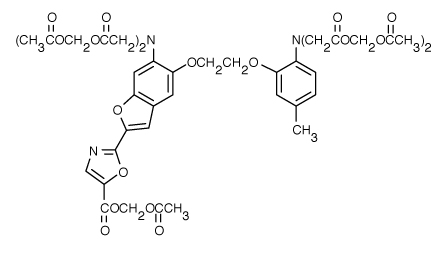
\includegraphics[scale=0.55]{Figures/fura2am.jpg}
	}
	\subfloat[CPA]{
	\label{fig:cpa}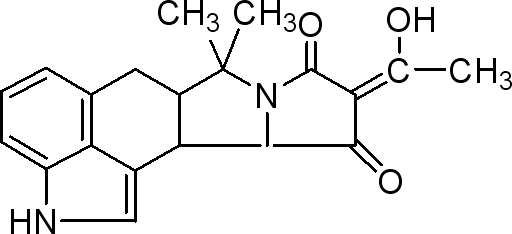
\includegraphics[scale=0.35]{Figures/CPA.jpg}
	} \\
	
	\subfloat[Probenecid]{
	\label{fig:probenecid}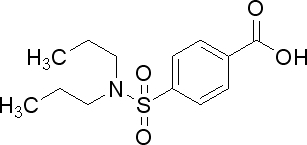
\includegraphics[scale=0.7]{Figures/probenecid.jpg}
	}\hspace{35pt} % ADD some HORIZONTAL SPACE TO ALIGN
	\subfloat[2-APB]{
	\label{fig:2apb}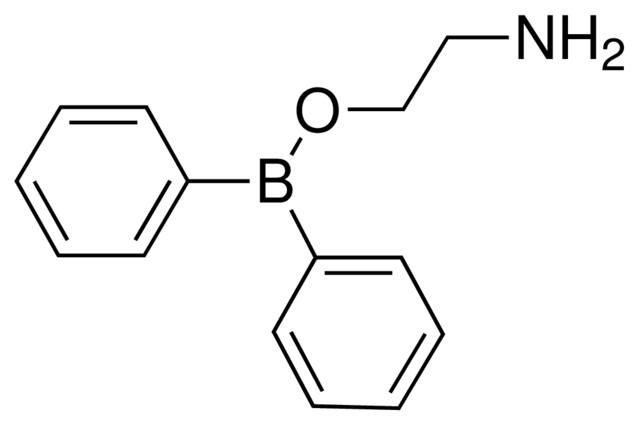
\includegraphics[scale=0.25]{Figures/2apb.jpg}
	}
	\caption{Structures of chemical reagents used in this study.}
\end{figure}

\subsection{2-Aminoethoxydiphenyl Borate}
2-aminoethoxydiphenyl borate (2-APB) (CAS Number: 524-95-8, (C$_6$H$_5$)$_2$BOCH$_2$CH$_2$NH$_2$) is a drug which has multiple effects on a variety of cellular organelles. It is an inhibitor of IP3Rs and SERCA pumps, and has both activating and inhibitory effects on channels \citep{Prakriya2001, Bilmen2002, Dellis2011}. As mentioned above, its effect on Orai1 channels is to activate them at concentrations $<$ 10 $\mu$M, while inhibiting at higher concentrations \citep{Prakriya2001,Feske2006,Gwack2007,Goto2010}. This dual effect is limited to Orai1, whereas for Orai3, 2-APB only activates at concentrations $\ge$ 50 $\mu$M \citep{Gwack2007}. 
%\todo{read Prakriya2001 for more information on 2-APB}
%This different responses to suggests that Orai3 interacts differently with 2-APB. 

Contrasting responses to 2-APB are often used to dissect functional differences in cells expressing multiple Orai isoforms \citep{Feske2006,Goto2010,Prakriya2006,Zhang2008a}. There is precedent then for the use of 2-APB to help extract useful information about Orai3. Obtaining even more information on Orai3 through the use of 2-APB is possible. If interactions between Orai3 channels and 2-APB are direct, crystal structures with 2-APB could help define the structure of this binding site. Such information may be helpful in finding the natural modulator of Orai3's SOCE activating function. It is evident then, that the question of whether Orai3 interacts directly with 2-APB is worthy of study. By expressing Orai3 in a \droso{} expression system, it becomes possible to obtain enough protein to do the type of crystallographic studies mentioned above. This study then can provide the foundation for future structural investigation, and its utility is not limited to pharmacological studies.

\subsection{Cyclopiazonic Acid}
Cyclopiazonic Acid (CPA) (CAS Number: 18172-33-3, C$_{20}$H$_{20}$N$_2$O$_3$) is an inhibitor of the endoplasmic reticulum's \Ca{} ATPase \citep{Moncoq2007}. It has been shown to be specific for the SERCA pump, and has been shown not to affect other ATPases or calcium pumps \citep{Moncoq2007}. The affinity of CPA for its substrate is $\sim$120 nM. The use of CPA allows for manipulation of SERCA pumps and, by extension, the ER \Ca{} store content \citep[chap. 2]{WPutney:2006p130}. Inhibition of the SERCA pump by CPA leads to release of the ER \Ca{} pools physiologically under the control of IP3R channels, \citep[chap. 2]{WPutney:2006p130}. 
 SERCA pump inhibition reveals a persistent \Ca{} leak from the ER, and makes it the predominant force driving \Ca{} movement. The result is an increase of cytoplasmic \Ca{} as it leaks from ER into cytoplasm. \Ca{} release occurs relatively quickly (minutes), as CPA is membrane permeant \citep{WPutney:2006p130}. 

CPA is added in a \Ca{} free solution containing a \Ca{} chelator. We then switch to a solution that contains \Ca{}, with no CPA. By emptying the cell's intracellular stores first, we may then reasonably assume that any subsequent increase in \cai{} is the result of \Ca{} entering the cell from the extracellular solution. 
 

\subsection{Ethylene glycol tetraacetic acid}
Ethylene Glycol Tetraacetic Acid (EGTA) is a cation chelator with a preference for \Ca{} over Mg$^{2+}$, Na$^+$ and K$^+$ %lambert, chap 1 
\citep{GLambert:2006p191}. It is used experimentally to bind available \Ca{} in the extracellular solution, making it unavailable for entry into the cell. This ensures that when \cai{} increases are observed during perfusion with an EGTA containing solution, we can assume that these increases are the result of intracellular \Ca{} release, and not extracellular \Ca{} entry \citep{GLambert:2006p191,WPutney:2006p130}.

\subsection{Fura-2}
The ability to measure \cai{} changes comes from the use of Fura-2. Fura-2 is a calcium indicator whose ability to bind calcium is the result of a negatively charged tetracarboxylic acid core. It is a BAPTA derivative, which in turn, is a modification of EGTA  \citep{GLambert:2006p191,WPutney:2006p130}. %lambert, chap 1

Fura-2 is a dual excitation indicator with a Kd of 145 nM for \Ca. At low [\Ca{}] excitation peaks at approximately 370 nm, while binding \Ca{} changes the excitation peak to 340 nm. Emission, meanwhile, is monitored at 510 nm. This results in \Ca{} binding leading to an increase in fluorescence at 510nm, when Fura-2 is excited at 340 nm. There is a corresponding decrease in fluorescence at 510 nm, when excited at 380 nm if \Ca{} is bound. By exciting both wavelengths in quick succession, \Ca{} binding changes can be monitored. This is referred to as a ratiometric approach, and has advantages over single-wavelength excitation (discussed in ref.\citealp{GLambert:2006p191}). %lambert, chap 1


The advantages are that the signal does not depend on the dye concentration, illumination intensity or optical path-length because we get normalized values from the ratios of the two wavelengths. Ratiometric measurements are therefore an improvement over the single-wavelength readings with respect to these issues as well. Dye leakage and photobleaching both lead to a loss of indicator during the experiment. In a single-wavelength setup, the dye concentration could gradually decrease, leading to a seeming decrease in \Ca{} signal. In the ratiometric setup, the effect of dye leakage or photobleached signals is mitigated by taking the ratios of these measurements. The ratios should remain constant regardless of the dye concentration or signal intensity. As an added advantage, ratiometric measurements increase sensitivity \citep{GLambert:2006p191, WPutney:2006p130}.  %lambert, chap 1

One noteworthy drawback is that Fura-2 fluorescence can be quenched by Cu$^{2+}$ \citep{WPutney:2006p130, Millar1995}. Since we use \cuso{} to induce gene expression in S2 cells, this is directly relevant to our study. Care therefore is taken with measurements from \cuso-induced S2 cells. These cells are spun down, washed in PBS, and then re-suspended in S2 media containing no \cuso{} to minimize quenching. % Also, EGTA binds Cu$^{2+}$ very well and removes any residual copper left

\subsubsection{Fura-2-AM}
\Ca{} indicators are, necessarily, charged molecules. In spite of this, we need them to cross the lipophilic PM. Since diffusional transport of these large, charged molecules across the lipophilic membrane would be extremely slow, other methods are used to speed up the process. By esterification of the -COOH groups of Fura-2, these groups are made lipophilic and thus membrane permeant. Indicators with these modifications are usually available as acetoxymethyl (AM) esters. Such is the case here, and the Fura-2-AM variant is used to load the dye into our S2 cells. 
Once inside the cell, cytosolic esterases are needed to remove the AM groups. Once these groups are removed, Fura-2 regains its charge, and may no longer freely cross the PM. 

One caveat of this method is that cell types with low esterase activity will display poor loading \citep{GLambert:2006p191}.  %lambert, chap 1
Another is that cellular processes, presumably designed to maintain ionic equilibrium, may pump the de-esterified, charged compound out of the cell. To combat this problem, the anion transporters responsible for this process can be blocked. This strategy was found to be necessary for S2 cells \citep{Cordova2003a, Yagodin1999}. Probenecid was used for this purpose in our study.


\subsection{Probenecid}
Probenecid (CAS Number: 57-66-9, C$_{13}$H$_{19}$NO$_4$S) is a nonspecific inhibitor of anion transport \citep{Cordova2003a, Masereeuw2000}. The reason for wanting to inhibit anion transport is to prevent cells from transporting the Fura-2 dye out of the cytosol. Many cell types are capable of sequestering the dye into different compartments, and also of transporting the dye out of the cell \citep{DiVirgilio1990}. There are a number of methods proposed for how Fura-2's cytosolic concentration could be reduced \citep{DiVirgilio1990, Cordova2003a}. Of those, the hypothesis that probenecid-sensitive anion transporters are responsible seems most plausible in \droso{} S2 cells \citep{Cordova2003a}. Murine macrophages have also shown a propensity for Fura-2 leakage \citep{DiVirgilio1990}. In the mouse macrophage model, the anion transporters were again implicated in Fura-2 leakage and blocking anion transport  prevented Fura-2 sequestration and secretion \citep{DiVirgilio1990}. It is easy to see then that S2 cells, which are also of macrophage origin, would have a similar response \citep{Schetz2004}.

\droso{} S2 cells have, in fact, been shown to exhibit poor loading of Fura-2, alleviated by probenecid \citep{Cordova2003a}. In our experiments we also experienced similar difficulties with loading the S2 cells in the absence of an anion blocker. Addition of 2.5 mM of probenecid alleviated this problem, increasing the number of cells loaded with Fura-2.

\subsubsection{The mode of action of Probenecid}
Probenecid is thought to act by inhibiting the clearance of ions \citep{Masereeuw2000}. 
It has also been reported that the drug has non-specific effects %, among them an altering of the 
on \Ca{} homeostasis \citep{Masereeuw2000}. 
Such information is important to be aware of, as \Ca{} measurements are the output from the experiments in our study. 
Care needs to be taken then, to ensure that the \Ca{} measurements would not be affected by probenecid. We address this by doing short 45-minute incubations in probenecid similar to other published studies \citep{Cordova2003a, Roos2005, Yagodin1999}, followed by washing these cells in our perfusion solution without probenecid.

Probenecid is soluble at basic pH. It is therefore dissolved in a solution of NaOH. This necessitates titrating the dye-loading solution back to the desired pH, after adding probenecid \citep{DiVirgilio1990}.  In mouse macrophage experiments, no unexpected effects on cell viability after a \emph{3-hour} incubation with probenecid were observed \citep{DiVirgilio1990}.  While there are caveats to its use, incubation at room temperature and for short periods, does not appear to affect cell function or viability \citep{Cordova2003a,DiVirgilio1990,Yeromin:2004p520}. 


\section{Specific Aims}
Before attempting to characterize human Orai3 \Ca{} channels in \droso{} S2 cells, we needed to create the insect vector which contained our mammalian GOI. Standard molecular biology techniques were used to achieve this. The pharmacological characterization was done by measuring the effect of 2-APB on heterologously expressed Orai3. We hypothesized that gene expression of mammalian Orai3 in \droso{} S2 cells would result in functional \Ca{} channels that behave similar to those in mammalian cells expressing Orai3 genes, when treated with 2-APB. 

\subsection{Specific Aim \#1}
As mentioned earlier, \droso{} S2 cells provide a good system for expressing proteins from other organisms. The \puchygmt{} vector was chosen to express our mammalian genes in S2 cells.  Specific aim \#1 is to create vector constructs using \puchygmt{} which express Orai3 and \stim{} in \droso{} S2 cells. 

\subsection{Specific Aim \#2}
After creating these vector constructs it will be necessary to determine if they are capable of supporting expression of the desired genes. Specific aim \#2 is to show that we can successfully express heterologous genes in \droso{} S2 cells.

\subsection{Specific Aim \#3}
It is our long term goal to ultimately use this system for drug discovery. For this to be possible we need to assess the effects which different drugs have in our system. This will be done using \Ca{} measurements taken in transiently transfected \droso{} S2 cells. Specific aim \#3 is to determine whether 2-APB has the same effect on the heterologously expressed Orai3 in S2s that it has in mammalian cells. 2-APB is a pharmacological agent with defined effects on the Orai3 \Ca{} channel. By looking at the effect of 2-APB on heterologously expressed Orai3, we will be able to determine whether the model requires refinement, or is suitable as is.

\section{Significance}
As stated above, Orai3 \Ca{} channels have been implicated in a specific subset of breast cancer. It is tempting to envision a scenario where we can specifically  target a type of breast cancer for treatment \citep{Dellis2011}. This will require some method to test the efficacy of drugs being used, however. If successful, creating a model system in \droso{} has the possibility to simplify drug testing, and as a result speed the process up. This could benefit research of, not only breast cancer, but also other disease states involving SOCE. Cancers, such as leukemia, and even autoimmune diseases such as rheumatoid arthritis or lupus, arising from defects of the immune system stand to benefit from this work. 

A successful \droso{} expression system provides benefits to biochemical analysis of Orai channels as well. Techniques such as x-ray crystallography require large amounts of protein. Such quantities are not easily achieved when working with mammalian cells, but become feasible with a \droso{} expression system. This study is also significant as it opens the possibility for extending the body of knowledge on Orai channels in both functional and structural fields of research.

% -eof-
